\section{Estructuras de datos relevantes}

En este apartado se detallan aquellas estructuras que son relevantes para realizar la gesti�n de datos del \textit{heap}.\\
Al final se tendr� una visi�n general de d�nde y c�mo se estructuran los datos que se almacenan en el \textit{heap} y, de este modo, conocer la manera en la que se gestionan los datos una vez se almacenan o liberan.
\bigskip

Los fragmentos de c�digo que se mostrar�n a continuaci�n se han extra�do de la versi�n 2.12.1 de la librer�a GNU est�ndar de C o, como se nombrar� en este documento a partir de ahora, \textit{glibc}. El c�digo fuente de la librer�a se puede encontrar en el enlace mencionado a pie de p�gina\footnote{La librer�a \textit{glibc} 2.12.1 se puede descargar de:\\ \url{http://ftp.gnu.org/gnu/glibc/glibc-2.12.1.tar.gz}}. \bigskip

Una vez descargado y descomprimido el archivo se podr� acceder al directorio \textit{glibc-2.12.1}. Dentro de este directorio examinaremos algunos de los archivos que se encuentran en la carpeta \textit{malloc} tales como \textit{malloc.c, malloc.h o arena.c}. Por otro lado, el directorio \textit{include}, dentro del directorio \textit{glibc-2.12.1}, contiene el archivo \textit{malloc.h} que tambi�n ser� de inter�s. A partir de ahora, siempre que se refiera a \textit{malloc.c, malloc.h o arena.c} se hace referencia a aquellos archivos ubicados en el directorio \textit{malloc} a menos que se especifique lo contrario.\bigskip

\subsection{Estructura heap\_info}

Un mismo proceso puede tener uno o varios \textit{heaps} dependiendo del n�mero de hilos - o \textit{threads} - del proceso. Es por esta raz�n que es necesaria una estructura que re�na y gestione este conjunto de \textit{heaps}. Esta estructura se conoce como \textit{heap\_info} y est� detallada en el C�digo \ref{code:heap_info_struct}. \bigskip

\lstset{language=C, caption=heap\_info (arena.c:59), label=code:heap_info_struct}
\begin{lstlisting}
typedef struct _heap_info {
  mstate ar_ptr;            /* Arena for this heap. */
  struct _heap_info *prev;  /* Previous heap. */
  size_t size;              /* Current size in bytes. */
  size_t mprotect_size;     /* Size in bytes that has been mprotected
                               PROT_READ|PROT_WRITE.  */
  /* Make sure the following data is properly aligned, particularly
     that sizeof (heap_info) + 2 * SIZE_SZ is a multiple of
     MALLOC_ALIGNMENT. */
  char pad[-6 * SIZE_SZ & MALLOC_ALIGN_MASK];
} heap_info;
\end{lstlisting}

\begin{itemize}
\item \textbf{ar\_ptr}
\begin{myindentpar}{1cm}
La primera variable |ar_ptr| es del tipo |mstate| y se conoce como \textit{arena pointer}. Este tipo est� definido en el c�digo ubicado en el fichero \textit{include/malloc.h} tal que as�:  

\lstset{language=C, caption=mstate (include/malloc.h:11), label=code:mstate_struct}
\begin{lstlisting}
struct malloc_state;
typedef struct malloc_state *mstate;
\end{lstlisting}

Como se puede ver, |malloc_state| y |mstate| son equivalentes.\\
|mstate| es un puntero a la estructura |malloc_state| y la estructura |malloc_state| est� definida en el archivo \textit{malloc.c} y debido a su importancia tambi�n se detallar� en este apartado.\\
La variable |ar_ptr| hace referencia a la estructura |malloc_state| que es donde se gestionan todos los datos que se almacenen en el \textit{heap}. Esta definici�n de los datos implica que la relaci�n entre \textit{arenas} y \textit{heaps} es de uno a uno.\bigskip

Tal y como ya se ha comentado, un proceso puede tener varios \textit{heaps}, as� que el proceso de uso de los \textit{heaps} se basa en que cuando un proceso necesita almacenar nuevos datos, se busca si existe alg�n \textit{arena} sin bloquear\footnote{Debido a que \textit{ptmalloc} est� implementado para aplicaciones \textit{multithreaded} algunas estructuras de memoria pueden estar bloqueadas con t�cnicas de gesti�n de memoria compartida.}, de ser as�, se utiliza para almacenar los nuevos datos, de no existir ning�n \textit{arena} sin bloquear, se crea un nuevo \textit{heap} y se almacenan los datos en su respectivo \textit{arena}. Esta t�cnica se utiliza para reducir la problem�tica conocida como \textit{lock contention}.\cite{MPIAMLE}
\end{myindentpar}

\item \textbf{prev}
\begin{myindentpar}{1cm}
Con la variable |prev| se gestionan todas las estructuras |heap_info| que se crean durante la gesti�n de la memoria din�mica de un proceso. Como ya se ha comentado, es posible que un mismo proceso tenga m�ltiples \textit{heaps}. Estos \textit{heaps} se gestionan a trav�s de una lista enlazada de estructuras |heap_info|[arena.c:106]. \\
Sin embargo, dicha variable s�lo se utiliza en tres partes del c�digo. La primera es la funci�n |new_heap| [arena.c:693] que crea un nuevo \textit{heap} y devuelve una variable de tipo |heap_info *|, con todo y con eso, la variable |prev| no se inicializa en dicha funci�n. La segunda parte es en la funci�n |heap_trim| [arena.c:840] y, de nuevo, en esta funci�n tampoco se inicializa la variable, s�lo se utiliza.
Finalmente, la variable |prev| se inicializa en la funci�n |sYSMALLOc| [malloc.c:2965] despu�s de llamar a la funci�n |new_heap|. Sin embargo, la funci�n |sYSMALLOc| s�lo se llama cuando las peticiones de almacenamiento de datos cumplen ciertos requisitos en cuanto al tama�o de los datos, y dichos requisitos pocas veces se cumplen [malloc.c:4747].\\
En pocas palabras, parece que esta variable se utiliza en situaciones marginales y la l�gica de su funcionamiento no es muy clara.
\end{myindentpar}

\item \textbf{size}
\begin{myindentpar}{1cm}
En la variable |size| se almacena el tama�o del propio \textit{heap}.
\end{myindentpar}
\end{itemize}

Tanto la variable |pad| como la variable |mprotect_size| no son relevantes y con los comentarios del c�digo fuente hay m�s que suficiente. \bigskip

\subsection{Arena}

La siguiente estructura a analizar es |malloc_state|. Esta estructura es la que se conoce como \textit{arena}. El c�digo que la define es el siguiente: \bigskip

\lstset{language=C, caption=malloc\_state (malloc.c:2362), label=code:malloc_state_struct}
\begin{lstlisting}
struct malloc_state {
  /* Serialize access.  */
  mutex_t mutex;

  /* Flags (formerly in max_fast).  */
  int flags;

#if THREAD_STATS
  /* Statistics for locking.  Only used if THREAD_STATS is defined.  */
  long stat_lock_direct, stat_lock_loop, stat_lock_wait;
#endif

  /* Fastbins */
  mfastbinptr      fastbinsY[NFASTBINS];

  /* Base of the topmost chunk -- not otherwise kept in a bin */
  mchunkptr        top;

  /* The remainder from the most recent split of a small request */
  mchunkptr        last_remainder;

  /* Normal bins packed as described above */
  mchunkptr        bins[NBINS * 2 - 2];

  /* Bitmap of bins */
  unsigned int     binmap[BINMAPSIZE];

  /* Linked list */
  struct malloc_state *next;

#ifdef PER_THREAD
  /* Linked list for free arenas.  */
  struct malloc_state *next_free;
#endif

  /* Memory allocated from the system in this arena.  */
  INTERNAL_SIZE_T system_mem;
  INTERNAL_SIZE_T max_system_mem;
};
\end{lstlisting}

\begin{itemize}
\item \textbf{fastbinsY[...]}
\begin{myindentpar}{1cm}
En la variable |fastbin|\footnote{A partir de ahora a la variable \textit{fastbinY} se la llamar� \textit{fastbin} ya que as� es como se conoce al concepto que define.} se almacenan fragmentos de memoria que se han liberado recientemente. Esta variable almacena dichos fragmentos de memoria y se utilizan en un orden |LIFO| por cuestiones de rendimiento a diferencia de los \textit{bins}\footnote{El concepto \textit{bin} se definir� a continuaci�n, por ahora basta con saber que con \textit{bin} se identifica a un espacio de memoria en el que almacenar y organizar los fragmentos de memoria asignados.} normales que se utilizan en un orden |FIFO| [malloc.c:2263].\\
Los fragmentos de memoria referenciados en la variable \textit{fastbin} mantienen su bit \textit{inuse}  [\ref{sec:memory_chunks}] a 1 de modo que estos fragmentos de memoria nunca se fusionan para crear un fragmento de memoria liberado m�s grande, a menos que se ejecute la funci�n |malloc_consolidate|[malloc.c:5088] que libera los fragmentos de memoria de los \textit{fastbins} y los fusiona con otros fragmentos de memoria libres [malloc.c:2271].\\
El tipo de la variable \textit{fastbin} es un puntero a |malloc_chunk| tal y como se define en [malloc.c:2277]:\bigskip

\lstset{language=C, caption=mfastbinptr (malloc.c:2277), label=code:mfastbinptr}
\begin{lstlisting}
typedef struct malloc_chunk* mfastbinptr;
\end{lstlisting}
La estructura |malloc_chunk| se estudiar� m�s adelante, sin embargo, se puede avanzar que dicha estructura identifica a un fragmento de memoria.\\
El n�mero de \textit{fastbins} viene definido por la constante |NFASTBINS|, que en el caso de una arquitectura de 32 bits  donde el tama�o del tipo |size_t| es de 4 bytes el valor de la constante es 10\cite{UTHBBI}.\bigskip

El objetivo de esta variable es el de tener acceso a peque�os fragmentos de memoria que est�n libres y a punto para poder almacenar datos de un modo eficiente. Esta estructura permite tener acceso a fragmentos de memoria libres de un modo eficiente, sin embargo, debido a que dichos fragmentos de memoria no se fusionan con otros fragmentos libres se incrementa el nivel de fragmentaci�n de la memoria.\bigskip 
\end{myindentpar}

\item \textbf{top}
\begin{myindentpar}{1cm}
La variable \textit{top} es de tipo |mchunkptr| que como se puede ver a continuaci�n no es m�s que un puntero a una estructura |malloc_chunk|:\bigskip
\lstset{language=C, caption=mchunkptr (malloc.c:1608), label=code:mchunkptr}
\begin{lstlisting}
struct malloc_chunk;
typedef struct malloc_chunk* mchunkptr;
\end{lstlisting}
La estructura |malloc_chunk| se estudiar� m�s adelante, sin embargo, se puede avanzar que dicha estructura identifica a un fragmento de memoria.\\
As� pues, la variable \textit{top} identifica un fragmento de memoria en especial que delimita el final de la memoria disponible del \textit{arena}. Este fragmento no est� almacenado en ning�n \textit{bin} y representa el espacio libre o sin asignar del propio \textit{arena}. S�lo se asigna espacio de memoria del \textit{top} cuando no hay ning�n otro fragmento de memoria libre [malloc.c:2217].
\end{myindentpar}

\item \textbf{last\_remainder}
\begin{myindentpar}{1cm}
Igual que la variable |top|, la variable |last_remainder| identifica un fragmento de memoria - |mchunkptr| - libre. Este fragmento de memoria es especial porque es el espacio restante cuando otro fragmento de memoria de poco tama�o se ha dividido para almacenar otros datos. Espec�ficamente, |last_remainder| apunta al �ltimo fragmento de poco tama�o dividido [malloc.c:2380].\\
El uso de la variable |last_remainder| se da en [malloc.c:4401].
\end{myindentpar}

\item\label{lab:bin_definition} \textbf{bins[...]}
\begin{myindentpar}{1cm}
\paragraph{}\label{par:bins}
La variable |bins| es un array que apunta a diferentes fragmentos de memoria |mchunkptr|. El objetivo de la variable |bins| es mantener una lista de varios fragmentos de memoria libres y de diferentes tama�os. En la mayor�a de los casos, cuando se haga una petici�n de memoria por parte del usuario, los datos se almacenar�n en alg�n \textit{bin} que est� disponible y que sea del tama�o adecuado. Es por esta raz�n que esta estructura es una de las m�s importantes. Existen un total de 128 \textit{bins} definidos por la constante |NBINS| [malloc.c:2162], sin embargo, el tama�o del array |bins| es de |NBINS| * 2 - 2, o sea, 254.\\
La variable \textit{bins} es un array, pero cada uno de estos \textit{bins} - o posiciones del array - identifica un fragmento de memoria que est� doblemente enlazado con otros fragmentos de memoria. As� pues, cada uno de los \textit{bins} apunta hacia una lista enlazada de fragmentos de memoria libres. De este modo, los fragmentos de memoria libres de los que dispone el proceso se organizan de un modo en el que su acceso es �ptimo. \\
Tal y como se especifica en el c�digo fuente [malloc.c:2141] existen los siguientes \textit{bins} con sus respectivos tama�os: \bigskip

\UndefineShortVerb{\|} %% Necesario para poner la barra vertical entre las filas de la tabla (linea 153).
\begin{table}[!htp]
	\topfigrule
   	\addtolength{\abovecaptionskip}{-12pt}   	
   	\caption{Tama�o de los bins}
   	\label{tab:bin_sizes}   		
	\begin{center}
	\begin{tabular}{c | c}
		\hline
		N�mero de bins & Tama�o del bin (bytes) \\
		\hline
		64 & 8 \\
		\hline
		32 & 64 \\
		\hline
		16 & 512 \\
		\hline
		8 & 4096 \\
		\hline
		4 & 32768 \\
		\hline
		2 & 262144 \\
		\hline
		1 & Lo que queda \\
		\hline
	\end{tabular}
	\end{center}
\end{table}
\DefineShortVerb{\|} 
\end{myindentpar}

\item \textbf{next}
\begin{myindentpar}{1cm}
Para puntualizar m�s que lo comentado en el c�digo de la estructura |malloc_state| esta variable mantiene una lista enlazada circular de los \textit{arenas} existentes [arena.c:510]. Se puede ver su inicializaci�n en [arena.c:944] cuando es necesario crear un nuevo \textit{arena}. De este modo se puede acceder a un \textit{arena} o a otro dependiendo de si dichos \textit{arenas} est�n siendo utilizados - y, por lo tanto, bloqueados - en el mismo momento en que se necesita hacer una reserva de memoria. \\
Evidentemente, debido a que enlaza otros \textit{arenas}, su tipo es un puntero a la estructura |malloc_state|.
\end{myindentpar}

\item \textbf{next\_free}
\begin{myindentpar}{1cm}
Esta variable es una lista de \textit{arenas} que supuestamente est�n libres. Sin embargo, en el c�digo malloc.c no se le da ning�n uso, o sea, que a efectos pr�cticos es como si no existiera. En el archivo de c�digo arena.c existe una funci�n llamada |get_free_list()| en la que se trabaja con dicha variable, sin embargo, esta funci�n tampoco se ejecuta en ninguna parte de malloc.c.
\end{myindentpar}

\end{itemize}

Las variables que no se han detallado, no son relevantes para comprender a grandes rasgos c�mo funciona la gesti�n de la memoria din�mica. Las variables |mutex|, |stat_lock_direct|, |stat_lock_loop| y |stat_lock_wait| tienen que ver con cuestiones de memoria compartida. La primera se encarga de bloquear el \textit{arena} cuando est� en uso y las dem�s sirven para generar estad�sticas sobre dichos bloqueos.\\
Por otro lado, el array |binmap[...]| sirve para saber si los \textit{bins} est�n vac�os o no. Utilizado por cuestiones de rendimiento cuando se ha de encontrar un \textit{bin} disponible.\\
Por �ltimo, las variables |system_mem| y |max_system_mem| sirven para saber cuanta memoria del sistema se ha almacenado en el propio \textit{arena}. \bigskip


\subsection{Fragmentos de memoria}
\label{sec:memory_chunks}

Los fragmentos de memoria - o \textit{malloc chunks} - es donde se almacenan los datos por los que el usuario ha pedido espacio. Esta estructura de memoria es una de las m�s importantes ya que dependiendo de c�mo se gestionen las operaciones que le afectan es posible que se introduzcan vulnerabilidades en el algoritmo. \bigskip

El c�digo que identifica a los fragmentos de memoria es el siguiente: \bigskip

\lstset{language=C, caption=malloc\_chunk (malloc.c:1809), label=code:malloc_chunk_struct}
\begin{lstlisting}
struct malloc_chunk {
  /* Size of previous chunk (if free).  */
  INTERNAL_SIZE_T      prev_size;
  /* Size in bytes, including overhead. */
  INTERNAL_SIZE_T      size;

  /* double links -- used only if free. */
  struct malloc_chunk* fd;
  struct malloc_chunk* bk;

  /* Only used for large blocks: pointer to next larger size.  */
  /* double links -- used only if free. */
  struct malloc_chunk* fd_nextsize;
  struct malloc_chunk* bk_nextsize;
};
\end{lstlisting}

Como se puede ver por los comentarios del C�digo \ref{code:malloc_chunk_struct}, hay datos de la propio estructura que s�lo se utilizan si el fragmento de memoria est� en cierto estado. Esto significa que dependiendo del estado en el que est� el fragmento de memoria, se tendr� una representaci�n ''pr�ctica'' u otra.\\
Un fragmento de memoria s�lo puede estar en dos estados. En uso o libre. Tal y como se ha explicado anteriormente, si el fragmento de memoria est� libre, su direcci�n se acabar� almacenando en un \textit{bin}. Si el fragmento de memoria est� en uso, el usuario obtendr� la direcci�n de memoria donde podr� almacenar sus datos. \bigskip

Un fragmento de memoria en uso tiene la representaci�n que se muestra en la Figura \ref{fig:malloc_chunk_in_use}.

\begin{figure}[!htbp]  
    \centering
    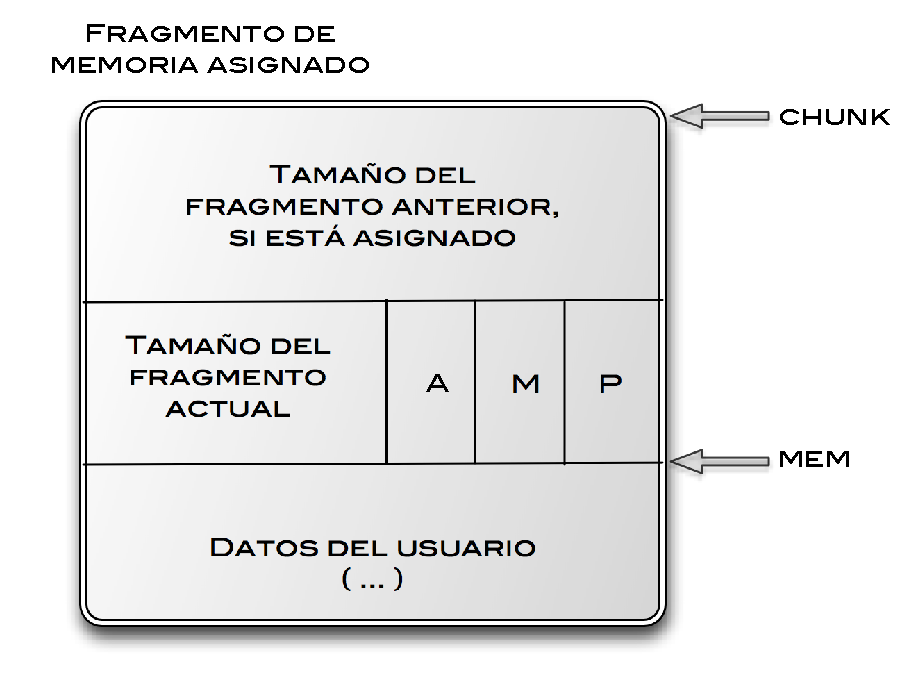
\includegraphics[scale=0.6]{./Chapters/HeapExploiting/HeapTheory/Estructuras/img/AllocatedChunk.eps}   
    \caption{Fragmento de memoria en uso}
    \label{fig:malloc_chunk_in_use}
\end{figure}

En la Figura \ref{fig:malloc_chunk_in_use} el puntero |chunk| apunta al principio del fragmento de memoria. La direcci�n de memoria a la que apunta |chunk| se utiliza por las rutinas internas del algoritmo. Adem�s, justo donde apunta |chunk| se encuentra el tama�o del fragmento de memoria, s�lo si dicho fragmento tambi�n est� en uso. \\
El siguiente campo de la estructura de datos es el tama�o del propio fragmento de memoria. Suponiendo una arquitectura de 32 bits, cada uno de estos campos es de 4 bytes, tal y como se puede comprobar a partir del tipo de cada campo: \bigskip

\lstset{language=C, caption=INTERNAL\_SIZE\_T (malloc.c:385), label=code:INTERNAL_SIZE_T}
\begin{lstlisting}
#ifndef INTERNAL_SIZE_T
#define INTERNAL_SIZE_T size_t
#endif
\end{lstlisting}

Por otro lado, los fragmentos de memoria siempre est�n alineados a un cierto valor. Esto se debe a que siempre que se hace una llamada a funciones como |malloc()|, el tama�o que se le pasa como argumento a la funci�n es substituido por un tama�o que cumpla ciertos requisitos tal y como se puede ver en las siguientes macros.\bigskip

\pagebreak

\lstset{language=C, caption=checked\_request2size (malloc.c:1955), label=code:checked_request2size}
\begin{lstlisting}
/* pad request bytes into a usable size -- internal version */

#define request2size(req)                                         \
  (((req) + SIZE_SZ + MALLOC_ALIGN_MASK < MINSIZE)  ?             \
   MINSIZE :                                                      \
   ((req) + SIZE_SZ + MALLOC_ALIGN_MASK) & ~MALLOC_ALIGN_MASK)

/*  Same, except also perform argument check */

#define checked_request2size(req, sz)                             \
  if (REQUEST_OUT_OF_RANGE(req)) {                                \
    MALLOC_FAILURE_ACTION;                                        \
    return 0;                                                     \
  }                                                               \
  (sz) = request2size(req);
\end{lstlisting}

Como se puede ver, la macro |checked_request2size| - que se ejecuta realizar al peticiones de memoria - devuelve 0 si el tama�o de la petici�n est� fuera de rango y de lo contrario, ejecuta la macro |request2size| que devuelve el tama�o correcto para la petici�n.\\
El tama�o devuelto ser� |MIN_SIZE| si el tama�o de la petici�n es menor al tama�o m�nimo permitido. Por contra si el tama�o es mayor al m�nimo aceptado, el tama�o devuelto ser� el tama�o de la petici�n, m�s |SIZE_Z|, m�s |MALLOC_ALIGN_MASK| y a este valor se le realizar� una \textit{and} l�gica con el valor de |MALLOC_ALIGN_MASK| negado. El valor de dichas constantes se puede ver a continuaci�n:\bigskip

\lstset{language=C, caption=SIZE\_SZ (malloc.c:392), label=code:SIZE_SZ}
\begin{lstlisting}
/* The corresponding word size */
#define SIZE_SZ                (sizeof(INTERNAL_SIZE_T))
\end{lstlisting}

La constante |SIZE_SZ| es igual a 4, ya que |INTERNAL_SIZE_T| equivale al tipo |size_t| que su tama�o en una arquitectura de 32 bits es 4.\bigskip

\lstset{language=C, caption=MALLOC\_ALIGN\_MASK (malloc.c:404), label=code:MALLOC_ALIGN_MASK}
\begin{lstlisting}
#ifndef MALLOC_ALIGNMENT
/* comments */
#define MALLOC_ALIGNMENT       (2 * SIZE_SZ)
#endif

/* The corresponding bit mask value */
#define MALLOC_ALIGN_MASK      (MALLOC_ALIGNMENT - 1)
\end{lstlisting}

Se deduce entonces que |MALLOC_ALIGNMENT_MASK| es 7, que en binario se representa como 111. De este modo, y volviendo al C�digo \ref{code:checked_request2size}, se obtiene que el tama�o devuelto en una petici�n de memoria que supere el m�nimo aceptado siempre ser� el tama�o inicial de la petici�n m�s 4 m�s 7 y lo m�s importante es que los �ltimos tres bits de dicho tama�o siempre ser�n 0 debido a la \textit{and} l�gica que se realiza con el valor de |MALLOC_ALIGN_MASK| negado, que es igual a 29 bits a 1 y los tres bits menos significativos a 0.\\
Gracias a esta estrategia se pueden utilizar los �ltimos 3 bits de campo que identifica el tama�o del fragmento de memoria como metadatos. As� pues, el bit menos significativo, |P|, de dicho campo sirve para identificar si el fragmento de memoria anterior al actual est� en uso. El siguiente bit |M| identifica si el fragmento de memoria actual se ha asignado a trav�s de la llamada al sistema |mmap()| y, por �ltimo, el bit |A| sirve para identificar si el fragmento de memoria actual est� en un \textit{arena} que no es el principal.\\
Para obtener toda esta informaci�n se utilizan las siguientes macros:\bigskip

\lstset{language=C, caption=Metadatos en el campo tama�o (malloc.c:1969), label=code:bit_logic}
\begin{lstlisting}
/* size field is or'ed with PREV_INUSE when previous adjacent chunk in use */
#define PREV_INUSE 0x1

/* extract inuse bit of previous chunk */
#define prev_inuse(p)       ((p)->size & PREV_INUSE)


/* size field is or'ed with IS_MMAPPED if the chunk was obtained with mmap() */
#define IS_MMAPPED 0x2

/* check for mmap()'ed chunk */
#define chunk_is_mmapped(p) ((p)->size & IS_MMAPPED)


/* size field is or'ed with NON_MAIN_ARENA if the chunk was obtained
   from a non-main arena.  This is only set immediately before handing
   the chunk to the user, if necessary.  */
#define NON_MAIN_ARENA 0x4

/* check for chunk from non-main arena */
#define chunk_non_main_arena(p) ((p)->size & NON_MAIN_ARENA)
\end{lstlisting}

Como se puede ver, en todos los casos se utilizan \textit{ands} l�gicas para obtener el valor deseado. Si el bit en cuesti�n est� a 1, cada una de las macros devolver� 1, en caso contrario, 0.\\
Por otro lado, para obtener el tama�o del fragmento de memoria se utiliza esta macro:\bigskip

\pagebreak

\lstset{language=C, caption=Tama�o de un fragmento de memoria (malloc.c:1969), label=code:chunk_size}
\begin{lstlisting}
#define SIZE_BITS (PREV_INUSE|IS_MMAPPED|NON_MAIN_ARENA)

/* Get size, ignoring use bits */
#define chunksize(p)         ((p)->size & ~(SIZE_BITS))
\end{lstlisting}

Por �ltimo, despu�s del tama�o del fragmento de memoria actual vienen los datos que el usuario ha decidido almacenar. El puntero |mem| apunta al principio de los datos del usuario y dicha direcci�n es la que se devuelve en las funciones que utiliza el usuario para pedir memoria.\bigskip

A continuaci�n se detalla c�mo es un fragmento de memoria libre, o mejor dicho, un fragmento de memoria que ha estado en uso pero que ya se ha liberado. Tal y como se ha explicado anteriormente, la estructura de datos es la misma que con un fragmento de memoria en uso, sin embargo, su representaci�n ''pr�ctica'' es diferente.\\
La Figura \ref{fig:malloc_free_chunk} muestra cual es su representaci�n.\bigskip

\begin{figure}[!htbp]  
    \centering
    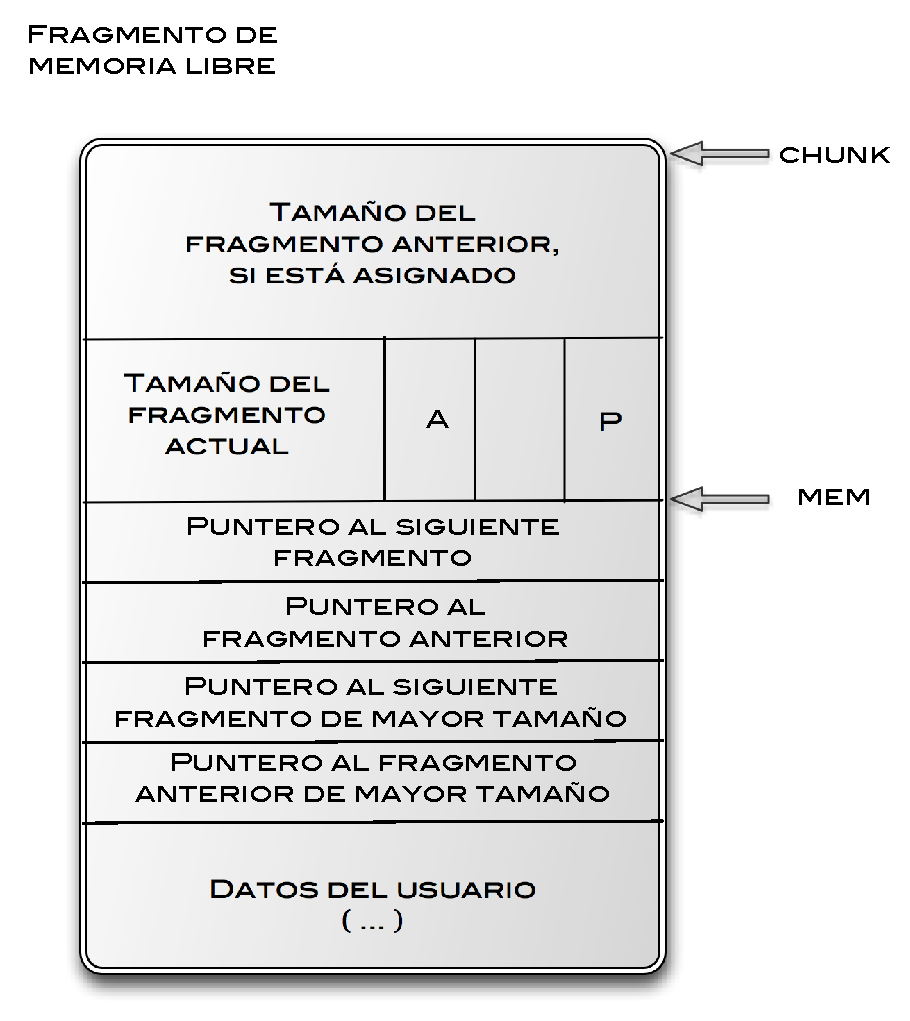
\includegraphics[scale=0.6]{./Chapters/HeapExploiting/HeapTheory/Estructuras/img/FreeChunk.eps}   
    \caption{Fragmento de memoria libre}
    \label{fig:malloc_free_chunk}
\end{figure}

De nuevo, en esta representaci�n aparecen los dos campos de tama�o, igual que con el fragmento de memoria en uso, sin embargo, esta vez el segundo bit menos significativo del campo que identifica el tama�o del fragmento actual ya no se utiliza. Esto se debe a que los fragmentos que se han reservado a trav�s de la llamada |mmap()|, una vez liberados, no se almacenan en ning�n \textit{bin} debido a que no hay listas que almacenen los fragmentos de memoria reservados con |mmap()|, sino que se liberan con |unmap()| [malloc.c:5060]. \bigskip

\paragraph{} \label{par:adjacent_chunks}
Un dato importante es que los fragmentos de memoria contiguos a este fragmento s�lo podr�n ser fragmentos de memoria en uso o el fragmento de memoria \textit{top}. Esto significa que nunca se tendr�n dos fragmentos de memoria libres contiguos ya que si este es el caso, estos dos fragmentos de memoria libres se fusionar�an en un s�lo fragmento [malloc.c:2070]. \bigskip

A continuaci�n de los campos de tama�o, se sit�an sendos punteros al pr�ximo y al anterior fragmento de memoria libre respectivamente. Es a partir de estos punteros con los que se navega en busca del fragmento de memoria libre que mejor se adec�e a la petici�n de memoria del usuario. \\
Un dato muy importante a tener en cuenta es que el puntero |mem|, que es la direcci�n de memoria que se le devolvi� al usuario a trav�s de una llamada, por ejemplo, a |malloc()| ahora apunta directamente a estos dos punteros.\bigskip

Despu�s existen otros dos punteros que identifican el siguiente y el anterior fragmento de memoria de un tama�o mayor al fragmento actual.\bigskip

Y por �ltimo, puede existir espacio libre que no se utiliza cuando el fragmento est� libre. \bigskip

\vspace*{5em}

Con los conocimientos expuestos en este cap�tulo es posible seguir adelante teniendo una base que permita entender los conceptos que se expondr�n a continuaci�n, sin embargo, cabe destacar que el funcionamiento de la gesti�n de la memoria din�mica es complejo y en estas escasas p�ginas no se han detallado ni mucho menos todas las funcionalidades de dicho algoritmo. Si bien es posible que en los siguientes cap�tulos se detallen conceptos b�sicos que no se han visto en este apartado.






\begin{comment}

Por �ltimo, la siguiente tabla contiene el tama�o de los fragmentos de memoria que se almacenan en cada uno de los \textit{fastbins}.
\begin{table}[!htp]
	\topfigrule
   	\addtolength{\abovecaptionskip}{-12pt}   	
   	\caption{Tama�o de los fragmentos almacenados en los fastbins}
   	\label{tab:fastbin_chunk_sizes}   		
	\begin{center}
	\begin{tabular}{||l | c | r||}
		\hline
		\hline
		# del fastbin & Tama�o del fragmento (bytes) & Tama�o real del fragmento (bytes) \\
		\hline
		0 & [0, 12] & 16\\
		\hline
		1 & [13, 20] & 24\\
		\hline
		2 & [21, 28] & 32\\
		\hline
		3 & [29, 36] & 40\\
		\hline
		4 & [37, 44] & 48\\
		\hline
		5 & [45, 52] & 56\\
		\hline
		6 & [53, 60] & 64\\
		\hline
		7 & [61, 68] & 72\\
		\hline
		8 & [69, 76] & 80\\
		\hline
		9 & [77, 80] & 88\\
		\hline
	\end{tabular}
	\end{center}
\end{table}

La primera columna representa el �ndice en el array de \textit{fastbins}. La segunda columna es el rango de tama�os te�ricos de los fragmentos de memoria que se pueden almacenar en cada uno de los \textit{fastbins} y la �ltima columna
\end{comment}